\chapter{First}

Other results I guess.

\chapter{Research Proposal}

\begin{center}
    \Large Application of a Non-variational Quantum Walk-based Optimisation Algorithm for Graph similarity

    \large Dylan O'Donoghue

    Supervisors: Tavis Bennett, Jingbo Wang

    May 26, 2024
\end{center}

\section{Introduction}
\subsection{Background}
Complex systems characterised by extensive interconnectivity, such as social networks, electrical power grids, circulatory systems, and database architectures are frequently modelled using network graphs \cite{databases}. Measuring the similarity between these graphs is crucial for enabling quantitative comparisons and gaining valuable insights. However, challenges arise when dealing with very large graphs, which significantly impact the scalability and efficiency of existing similarity algorithms. Moreover, the graph similarity problem becomes computationally intractable (requiring exponential time) for graphs without known labelling using conventional methods \cite{how_similar}. This project aims to address these challenges by exploring the application of the non-variational quantum walk-based optimisation algorithm (non-variational QWOA) \cite{bennett2024nonvariational}, potentially offering a breakthrough in solving the graph similarity problem more efficiently and effectively.

\subsection{Literature Review}
Network graph models have become crucial components in systems that are used in everyday life, such as search engines and social networks \cite{social-networks}. Graph similarity (or graph distinguishability, as it is sometimes referred \cite{quantum-distinguishability}) is often important in these contexts. For example, social networks are compared to identify certain interaction patterns \cite{citation-space}, traffic networks are compared to help detect abnormal changes in traffic patterns \cite{traffic}, and web networks are compared for anomaly detection \cite{web-anomalies}. In all these cases, the similarity between two graphs with overlapping sets of nodes is assessed and the detection of changes in the patterns of connectivity is important. For graphs which match approximately, it is useful to obtain a quantitative measure of similarity. For example, classification techniques in machine learning match objects that are within a certain tolerance.

Graph similarity measures are quantitative calculations based on comparisons made between the structure of network graphs. Different measures of graph similarity will produce a variety of results due to differences in how the structures of the graphs are analysed. There are many measures of graph similarity, including Maximum Common Subgraph \cite{MCS}, Graph Edit Distance \cite{GED}, Frobenius Distance \cite{frobenius-distance}, and Graph Eigendecomposition \cite{eigendecomposition}. These measures are all successful at indicating the degree to which two graphs are similar and can also detect small differences between them. 

\textbf{Graph similarity in detail:}

Let $G_{1}(V,E_{1} ), G_{2}(V,{E}_2)$ be two graphs defined by a set of vertices $V$ and edge sets $E_{1},E_{2}$. Define $sim(G_{1},G_{2} )\in[0,1]$ as the similarity of these graphs and define $A_{1},A_{2}$ as the adjacency matrices of $G_{1}$ and $G_{2}$, respectively. 

Koutra et al. formalised a set of axioms that graph similarity measures should conform to \cite{deltacon}:
\begin{enumerate}
    \item Identity: $sim(G_{1},G_{2})=1 \iff G_{1} \cong G_{2}$
    \item Symmetric:  $sim(G_{1},G_{2})=sim(G_{2},G_{1})$
    \item Zero: For a clique graph $G_{1}$ and a empty graph $G_{2}$, $sim(G_{1},G_{2}) \rightarrow 0 \text{ as } n\rightarrow \infty$ 
\end{enumerate}

They also raise that similarity algorithms should factor in the structural importance of each edge, the weight of removed edges, and the total number of edges in a graph. They also say a good graph similarity measure should be able to distinguish targeted and random changes, and should be scalable to large, generated graphs. However, this scalable criterion has only been fulfilled by algorithms applied to graphs with known node correspondence.

The failure of the scalability criterion for algorithms applied to graphs with unknown node correspondence (hereafter referred to as unlabelled graphs) is due to problem of finding the correct corresponding vertex labels between the graphs. Observe that due to Axiom 1, similarity algorithms should be able to identify isomorphic graphs (and assign them a similarity of 1), but confirming isomorphism requires checking each permutation of vertex labelling. Using this fact, the similarity of an unlabelled $G_{1}$ and $G_{2}$ can be expressed as:
$$
sim(G_{1},G_{2})=\underset{\pi}{\text{max }}simscore(A_{1}^{\pi},A_{2})
$$
Here, $\pi$ ranges over all permutations of the vertex set $V$, $A_{1}^{\pi}$ denotes the adjacency matrix obtained from $G_{1}$ by permuting rows and columns according to $\pi$, and $simscore$ is a function that assigns a scalar in the range $[0,1]$, called the similarity score, to a particular pair of adjacency matrices. The structure of $simscore$ depends on the measure of graph similarity that is being used. Note that in this scope, the graph similarity problem is the problem of finding the optimal alignment of two graphs such that their similarity score is maximised.

Since the unlabelled graph matching problem is NP-complete \cite{how_similar}, existing algorithms to measure graph similarity take exponential time to compute. Therefore, it is desirable to use quantum algorithms.

\textbf{Quantum Optimisation Algorithms:}

Using the previously established framework, we can reduce the problem of graph similarity to a combinatorial optimisation problem (COP) suitable for quantum algorithms. The COP consists of $n$ integer decision variables $x_{i}\in \{0,1,2,...,n-1 \}$ where the solutions are characterised by vectors $\mathbf{x}=(x_{1},x_{2},...,x_{n})$, which represent a particular labelling of vertices of $G_{1}$ onto $G_{2}$ (similar to $A_{1}^{\pi}$), and the space of feasible solutions $S$ contains all such vectors without repeating elements, such that there are $N$ feasible solutions where $N=n!$.  The system is initially in an equal superposition of all solutions,
$$
\ket{s} = \frac{1}{\sqrt{N}} \sum \ket{\mathbf{x}},
$$
and we seek to amplify the probability of measuring the solution $\mathbf{x}$ that maximises $f(\mathbf{x})$, where $f$ is the objective function that represents the equivalent $simscore$ for a particular $\mathbf{x}$.

One potential quantum algorithm that could be used is the quantum approximate optimisation algorithm (QAOA) \cite{QAOA}, which uses a variational approach to solving COPs. The algorithm repeatedly applies two Hamiltonians to $\ket{s}$, where the application times of each Hamiltonian are classically controlled parameters. These parameters are initially random and must be tuned via a classical optimisation process. The parameters that globally maximise the expected value of the objective function must be selected for optimal performance of the algorithm \cite{QAOA-review}.

Another variational algorithm is the quantum walk-based optimisation algorithm (QWOA), which is closely related to the main algorithm of this project. The QWOA is a more general form of the QAOA, where the time-based application of the transverse-field Hamiltonian is replaced by a continuous-time quantum walk (CTQW) on a graph that contains basis states encoding the feasible solutions to the COP \cite{QWOA}. The other Hamiltonian is unchanged and phase-shifts basis states depending on their associated objective function values.

The first concern in the use of variational algorithms is that the process of tuning the parameters is costly. The requirement to globally maximise these parameters means that gradient-based methods are more sensitive to the initial parameters, but the space of possible initial parameters grows exponentially in parameter count \cite{QAOA-optimiser}. In essence, variational algorithms solve the maximisation of the objective function, but also present the challenge of solving the maximisation problem of their own parameters. As such, a non-variational approach is preferred for our problem.

Another problem with the above algorithms is that they are built on a quadratic unconstrained binary optimisation (QUBO) framework, and as such, the decision variables $x_{i}$ must be binary. This conflicts with the structure of the graph similarity problem, which requires the use of non-binary decision variables. Although studies have shown that non-binary problems can be implemented into the QUBO framework \cite{QUBO-traveling}, it requires introducing a penalty component to the objective function, further increasing the number of parameters.  As such, an approach not restricted to only binary decision variables is preferred.

To address these issues, this project will implement a non-variational, non-binary-restricted quantum algorithm.

\textbf{The Non-variational Quantum Walk-based Optimisation Algorithm:}

The main algorithm of this project is the non-variational quantum walk-based optimisation algorithm (non-variational QWOA) \cite{bennett2024nonvariational}, which replaces the QWOA CTQW graph with a mixing graph that connects nearest-neighbour solutions.

For the graph similarity problem, the mixing graph connects each solution state to the set of $\frac{1}{2}n(n-1)$ possible transpositions (obtained by swapping two elements in $\mathbf{x}$). As such, the adjacency matrix of the mixing graph can be expressed as
$$
A = \sum_{i=0}^{n-2} \sum_{i+1}^{n-1} \text{SWAP}_{i,j},
$$
where $\text{SWAP}_{i,j}$ is defined as the permutation matrix associated with swapping the $i^{\text{th}}$ and $j^{\text{th}}$ entry in $\mathbf{x}$ and applying identity to the remaining entries.

There are two important unitaries driving the interference process in the non-variational QWOA. The first is the phase-separation unitary,
$$
U_{Q}=e^{-i\gamma Q}.
$$
$Q$ is the quality, a diagonal operator such that $Q\ket{\mathbf{x}}=f(x)\ket{\mathbf{x}}$. Hence, the phase-separation unitary applies a phase-shift to each solution state proportional to its objective function value. 

The second unitary is called the mixing unitary or mixer, and it performs the CTQW for time $t$ on the mixing graph,
$$
U_{M}= e^{itA}.
$$
After establishing these unitaries and given a pre-selected number of iterations $p$, the amplified state is defined as:
$$
\ket{\gamma,t,\beta}=\left[\prod_{j=0}^{p-1} U_{M}(t_{j}) U_{Q}\left(\frac{\gamma_{j}}{\sigma} \right) \right] \ket{s}
$$
Where $\gamma$, $t$, and $\beta$ are classically controlled positive-valued parameters that determine the applied phase separations and mixing times for each iteration. The values of $\gamma_{j}$ increase linearly over the domain $[\beta \gamma , \gamma]$, and the values of $t_{j}$ decrease linearly over the domain $[\beta t,t]$. $\sigma$ is standard deviation of $f(x)$, controlling the different possible measures of graph similarity such that $\gamma \approx 1$. An approximate value of $\sigma$ is sufficient and so can be found through random sampling of $f(\mathbf{x})$. An appropriate value of $\beta$, which is in the interval $(0,1)$, is unique to a particular problem type. As such, it is expected that once found, a single value of $\beta$ will be suitable for all graph similarity problems. Notably, Bennett et al. observes that optimal values of $\beta$ range from approximately $0.4$ down to $\frac{1}{p}$ for the problems of Weighted Maxcut, Maximum Independent Set, K-Means Clustering, Capacitated Facility Location, and the Quadratic Assignment Problem \cite{bennett2024nonvariational}.

\section{Project}
\subsection{Aims}
The primary goal of this project is to explore the uses of the non-variational QWOA for computing graph similarity, particularly investigating how modifications to the objective function and parameter tuning method influence the performance.

Secondary goals include benchmarking the performance of the algorithm using high performance computing (HPC) resources as well as generalising the implementation of the algorithm to work on weighted graphs, directed graphs and graphs with differing numbers of nodes. Additionally, I may show a proof-of-concept application of the algorithm on a practical case, such as small social network similarity.

\subsection{Significance}
This numerical simulation project is part of a larger project to benchmark the non-variational QWOA across various combinatorial optimisation problems. The non-variational QWOA has shown promising preliminary results, which may indicate that it is a practical quantum algorithm that could outperform equivalent classical or quantum methods. By contributing to the development and benchmarking of the non-variational QWOA, this project aims to advance the field of quantum computing and algorithms, potentially impacting areas such as network security, design, and logistics.

\section{Research Plan}
\subsection{Methodology and Problems}
The code developed to run the numerical simulations on local hardware is in Python, due to the need for high clarity and readability to perform investigations of the performance of the non-variational QWOA. An important aspect of this part of the project is the ability to rapidly prototype the simulation in response to the obtained results. The performance of the code on local hardware is not high priority, as the number of qubits a serial program is able to simulate is highly restricted anyway. The HPC benchmarking simulations will be run on the supercomputer Setonix, at the Pawsey Supercomputing Centre, and the best programming language for these benchmarking simulations will be identified as part of the project.

To analyse the effect of changing the measure of graph similarity, the objective function of the non-variational QWOA will be modified to reflect the required calculation associated with the $simscore$ for various measures of graph similarity. Comparisons between the performance of the algorithm using different measures of graph similarity will be used to explore how the algorithm is affected by changes in the measure of graph similarity.

The method by which the $\gamma, t,$ and $\beta$ parameters are tuned will also be an area of inquiry. This will involve investigating which tuning method produces the greatest amplification in the optimal solution state, as well as attenuation on the non-optimal solution states.

A potential problem that may arise in benchmarking is that due to the overhead that quantum algorithms require, the benefit of a speed up is normally only achieved for problems with a large size $n$. Thus, the size of the benchmarking simulations would likely need to have a large $n$. This may involve excessive time or resources which could cause problems with the size of the scope of the project.
\subsection{Preliminary Work}
This semester I have focused on building an in-depth understanding of the non-variational QWOA and similar quantum algorithms. Additionally, I have worked on obtaining preliminary results, building on the code originally developed by Tavis Bennett. 

A graph $G_{1}$ was randomly generated using an Erdös-Rényi random graph model \cite{erdos_renyi} with $N=9$ nodes and probability for edge inclusion  $p=0.5$. The second graph $G_{2}$ was a copy of the first graph, but with a single edge removed. The implemented objective function was the number of matching entries in the adjacency matrices of the graphs, divided by the total number of entries in the adjacency matrix. Since only one edge was different between $G_{1}$ and $G_{2}$, that meant two entries in the adjacency matrices $A_{1}$ and $A_{2}$ differed, giving an expected similarity of $\frac{79}{81}\approx 0.97$

I tuned the $\gamma, t,$ and $\beta$ parameters using two different methods. The first tuning method selected the parameters that would maximise the expected value of the objective function, $\langle f(x)\rangle$. The second tuning method selected the parameters that would maximise the probability to measure the optimal solution state, $P(\text{opt})$. These methods produced the values shown in Table \ref{table:1}.

\begin{table}[ht]
    \centering
    \begin{tabular}{|c|c|c|c|}
        \hline
        Tuning Method & $\gamma$ & $t$ & $\beta$\\
        \hline
        $\langle f(x)\rangle$ & 1.4745 & 0.2194 & 0.3545\\
        \hline
        $P(\text{opt})$ & 1.2378 & 0.2269 & 0.6568\\
        \hline
    \end{tabular}
    \caption{Optimal parameter values from different tuning methods }
    \label{table:1}
\end{table}

Using these values for the parameters, numerical simulations of the non-variational QWOA was applied to $G_{1}$ and $G_{2}$ with a number of iterations $p=10$, and the plots \ref{fig:image1}, \ref{fig:image2}, and \ref{fig:image3} were created.

Using these values for the parameters, numerical simulations of the non-variational QWOA was applied to $G_{1}$ and $G_{2}$ with a number of iterations $p=10$, and the plots \ref{fig:image1}, \ref{fig:image2}, and \ref{fig:image3} were created.

\begin{figure}[ht]
\begin{subfigure}{0.45\textwidth}
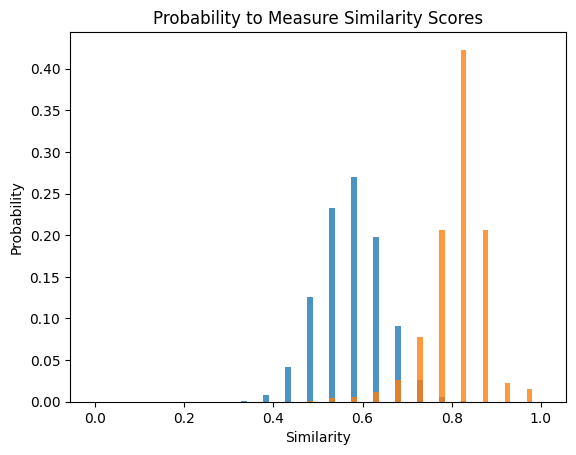
\includegraphics[width=0.9\linewidth,]{styles/mu_tuning_scores.png} 
\caption{Tuned by $\langle f(x)\rangle$}
\label{fig:subim1}
\end{subfigure}
\begin{subfigure}{0.45\textwidth}
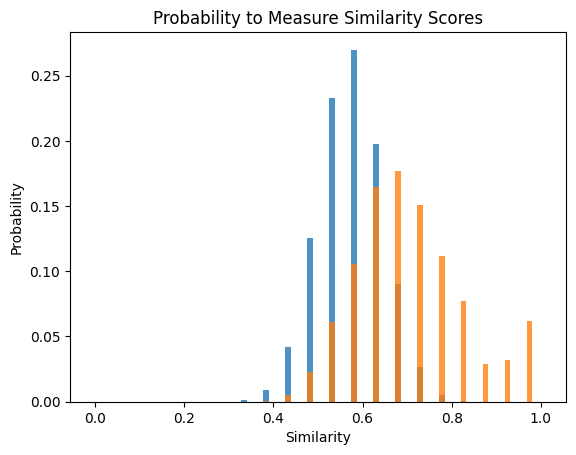
\includegraphics[width=0.9\linewidth]{styles/opt_tuning_scores.png}
\caption{Tuned by $P(\text{opt})$}
\label{fig:subim2}
\end{subfigure}
\caption{Similarity score probability distributions for different tuning methods.}
\label{fig:image1}
\end{figure}


\begin{figure}[ht]
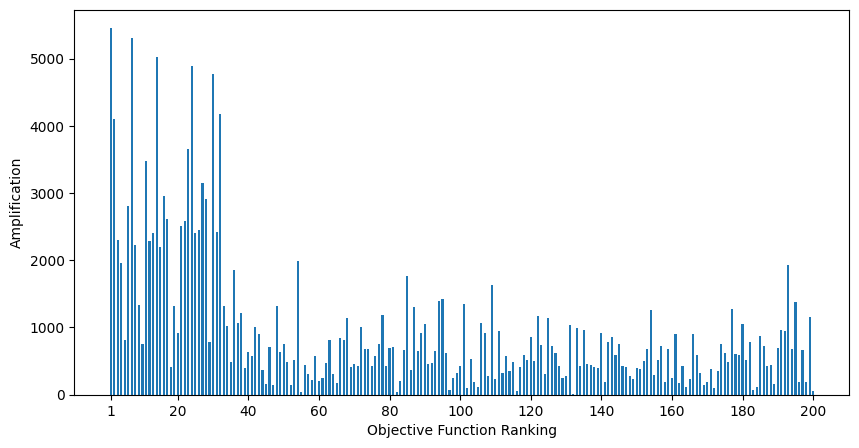
\includegraphics[width=0.9\linewidth]{styles/mu_tuning.png} 
\caption{Amount of amplification applied to the top 200 solutions when tuned by $\langle f(x)\rangle$}
\label{fig:image2}
\end{figure}

\begin{figure}[ht]
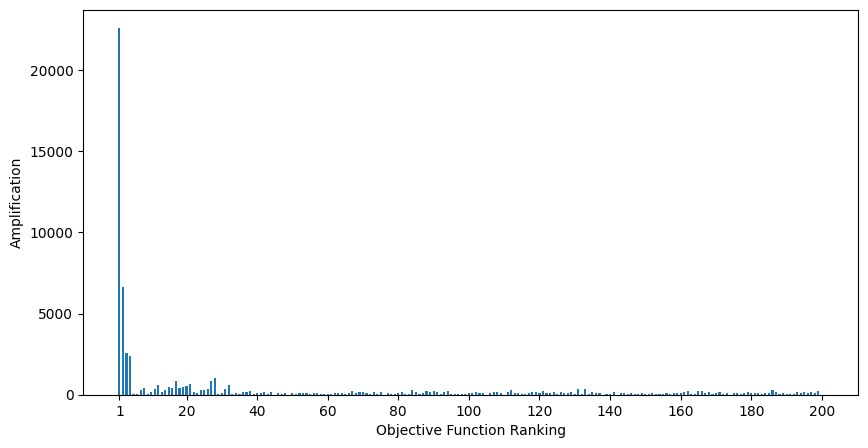
\includegraphics[width=0.9\linewidth]{styles/opt_tuning.png}
\caption{Amount of amplification applied to the top 200 solutions when tuned by $P(\text{opt})$}
\label{fig:im3}
\label{fig:image3}
\end{figure}

These plots show that for both tuning methods, the optimal solution was successfully amplified more than any other solution. However, the results also reveal several concerns. Firstly, we expect that tuning for $\langle f(x)\rangle$ and tuning for $P(\text{opt})$ should yield similar parameters, yet they produce very different $\beta$ values in Table \ref{table:1}. Bennett et al. suggest that $\beta$ should be $\approx 0.4$ or less, but the value of $\beta$ obtained from tuning for $P(\text{opt})$ significantly exceeds this guideline.

Secondly, when tuning for $\langle f(x)\rangle$, the amplification of non-optimal solutions is extremely high. The distribution of amplification in \ref{fig:image2} is spread out, and the amount of amplification applied to the optimal solution is much lower than in \ref{fig:image3}.

Finally, as a result of these previous behaviours, the most likely similarity score to measure from both simulations is not the similarity score corresponding to the optimal solution. 

All of these behaviours warrant further investigation into the configuration of the non-variational QWOA and adaptation of the tuning process is recommended to better align the results with theoretical predictions and practical requirements.